	\documentclass[12pt,letterpaper]{article}

\usepackage[spanish, es-tabla, es-nodecimaldot]{babel}
\usepackage[utf8]{inputenc}
\usepackage{amsmath}

\usepackage{hyperref}
\usepackage{url}
\usepackage{textcomp}
\usepackage{gensymb}
\usepackage[dvipsnames]{xcolor}

\usepackage{parskip}
\usepackage{fancyhdr}
\usepackage{multicol}
\usepackage{vmargin}
\usepackage{setspace}
\usepackage{geometry}

\usepackage{float}
\usepackage{array}
\usepackage{graphicx}
\graphicspath{{Images/}}
\usepackage{wrapfig}
\usepackage{caption}
\usepackage{subcaption}

\usepackage{listings}
\usepackage{color}
%\usepackage[usenames,dvipsnames]{color}
	\definecolor{ocre}{RGB}{42,105,21}
	\definecolor{ocre2}{RGB}{0,102,0}%47,109,130}
	\definecolor{gray2}{gray}{0.95}
	\lstset{
		language={[03]Fortran},
		backgroundcolor=\color{gray2},
		basicstyle=\color{black}\small\ttfamily, 
		breakatwhitespace=false,         
		breaklines=true,                 
		captionpos=b,                    
		columns=flexible,
		commentstyle=\color{ocre2}\ttfamily, 
		deletekeywords={...},            
		escapeinside={\%*}{*)},          
		extendedchars=true,             
		frame=single,	                 
		keepspaces=true,                 
		keywordstyle=\color{blue}\bfseries,       
		otherkeywords={*,...},          
		numbers=left,                    
		numbersep=5pt,                   
		numberstyle=\small, 
		rulecolor=\color{black},         
		showspaces=false,                
		showstringspaces=false,          
		showtabs=false,                  
		stepnumber=1,                    
		stringstyle=\normalfont\color{ocre},     
		tabsize=2,	                     
		title=\lstname                  
		}
\definecolor{labelcolor}{RGB}{100,0,0}



\setmarginsrb{2.0cm}{1.0cm}{2.0cm}{2.5cm}{0.5cm}{1cm}{1 cm}{1 cm} %{izq}{up}{der}{down}{Encabezado}

\pagestyle{fancy}
\fancyhf{}
\rhead{Lic. Física}
%\lhead{\thesection}
\cfoot{\thepage}


\title{ Comentarios, Desarrollos u Observaciones  }

\begin{document}


\begin{titlepage}
	\centering
    \vspace*{2cm}
	{\Huge Comentarios, Desarrollos u Observaciones \par}
	\vfill
	{\Large Desarrollo Experimental II \par}
	\vfill
	{\large\ Docente: Dra. Laura Lorenia Yeomans Reyna \par}
    \vfill
    {\large\ \textbf{Portafolio II}:\\ Simulación de Monte Carlo \par}
    \vfill
    {\large\ Martín Alejandro Paredes Sosa \par}
	\vfill
	% Bottom of the page
	{\large Semestre: 2018-1\par}
\end{titlepage}
\section*{Tarea III: Ejercicios para movimientos arbitrarios de partículas, condiciones periódicas y energía de la configuración }
A continuación se muestran los comentarios y avances relacionados con la tarea 3 del portafolio II.
\vspace{-0.5cm}

\subsection*{Actividad 1: Sin Condiciones Periódicas}
La actividad consistió en realizar el movimiento de partículas de manera aleatoria, sin considerar condiciones periódicas, es decir la partículas no vuelven a entrar a la celda. 
	\begin{figure}[H]
		\centering

		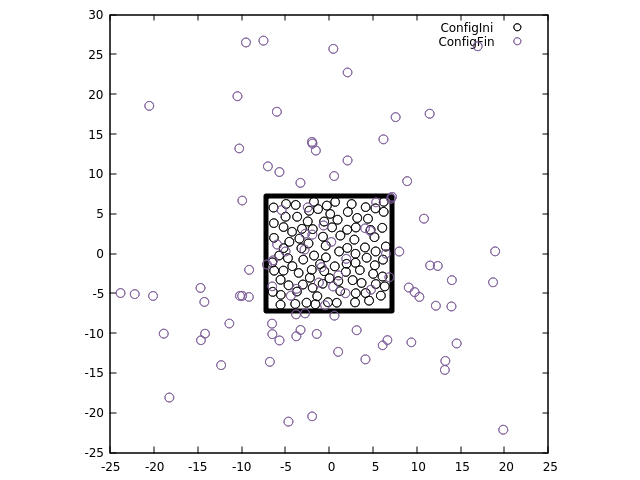
\includegraphics[scale=0.75]{Config_INI_FIN_2.png}
		\caption{Configuración Inicial con $n^*=0.5093$, con un $NStep=1000$ y un $\delta_{MAX}=0.5\sigma$}
	\end{figure}
	Se observa que las partículas se alejan consideradamente de las fronteras de la celda original.

\subsection*{Actividad 2}
La actividad consistió en realizar el movimiento de partículas de manera aleatoria, ahora considerando condiciones periódicas, es decir la partículas vuelven a entrar a la celda, cuando una sale, así asegurando que la concentración en la celda original se mantiene.
\begin{figure}[H]
		\centering
		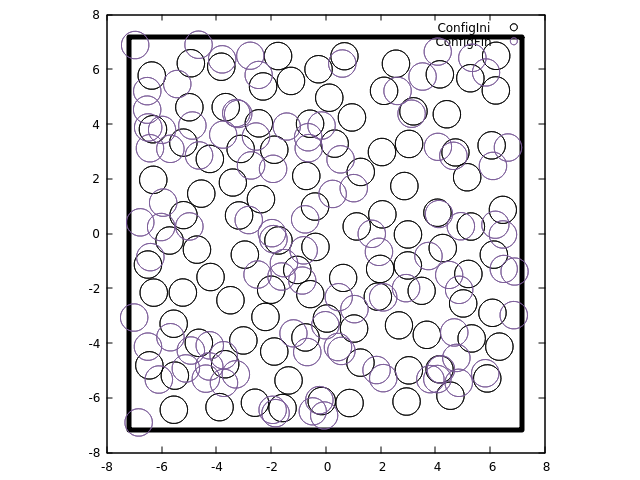
\includegraphics[scale=0.75]{Config_INI_FIN}
		\caption{Configuración Inicial con $n^*=0.5093$, con un $NStep=1000$ y un $\delta_{MAX}=0.5\sigma$}
	\end{figure}
Se observa que todas las partículas están dentro de la celda original, ligeramente afuera pero sus centros siguen dentro de las fronteras. 

Estas dos actividades permiten observar la forma en la que se mueven las partículas. La aplicación de condiciones periódicas es sencillo de implementar ya que consiste en volver a ingresar una partícula de lado opuesto de donde salio la otra.
\subsection*{Actividad 3}
La tercera actividad consistió en seguir el movimiento de dos partículas aleatorias. Esto permite observar las condiciones periódicas en acción.

	\begin{figure}[H]
		\centering
		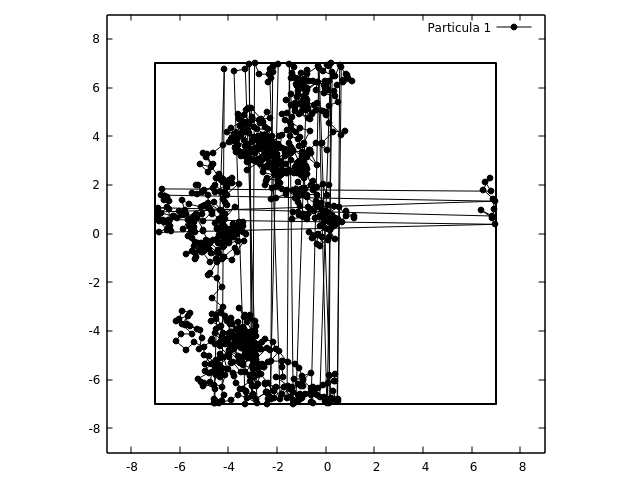
\includegraphics[width=0.49\linewidth]{Particula1.png}
		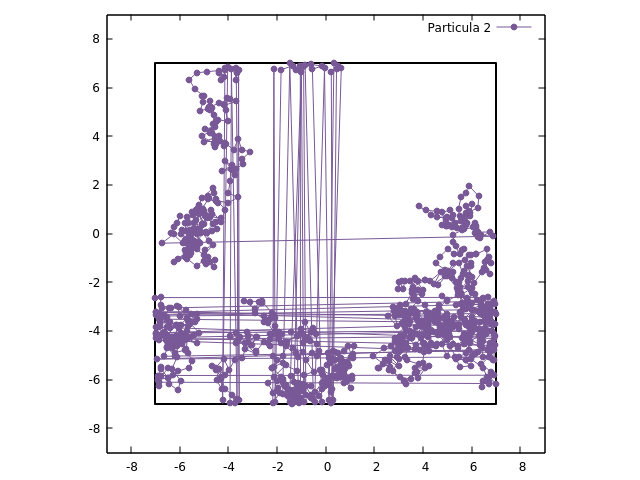
\includegraphics[width=0.49\linewidth]{Particula2.png}\\
		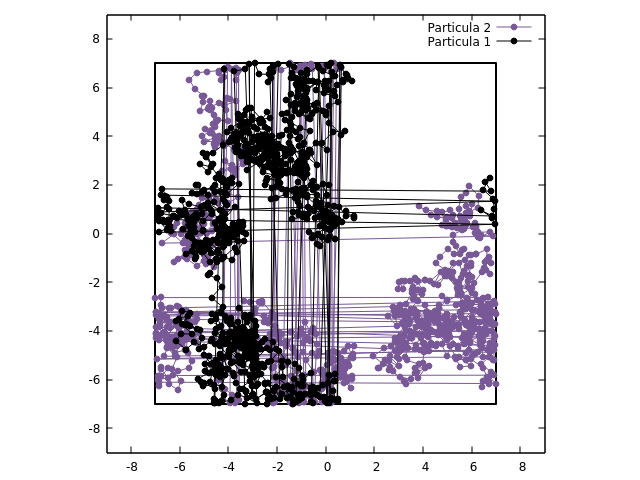
\includegraphics[width=0.75\linewidth]{Traza.png}
		\caption{ Con $n^*=0.5093$, con un $NStep=1000$ y un $\delta_{MAX}=0.5\sigma$. Se realizo la traza de las partículas 84 y 57.}
	\end{figure}
Se aprecia como cuando una partícula sale de las fronteras de la celda esta entra de lado opuesto cuando aparecen las lineas largas que atraviesan la celda.

\subsection*{Actividad 4}
La cuarta actividad consistió en realizar lo mismo que las actividades anteriores solo que adaptando a tres dimensiones.
	\begin{figure}[H]
		\centering
		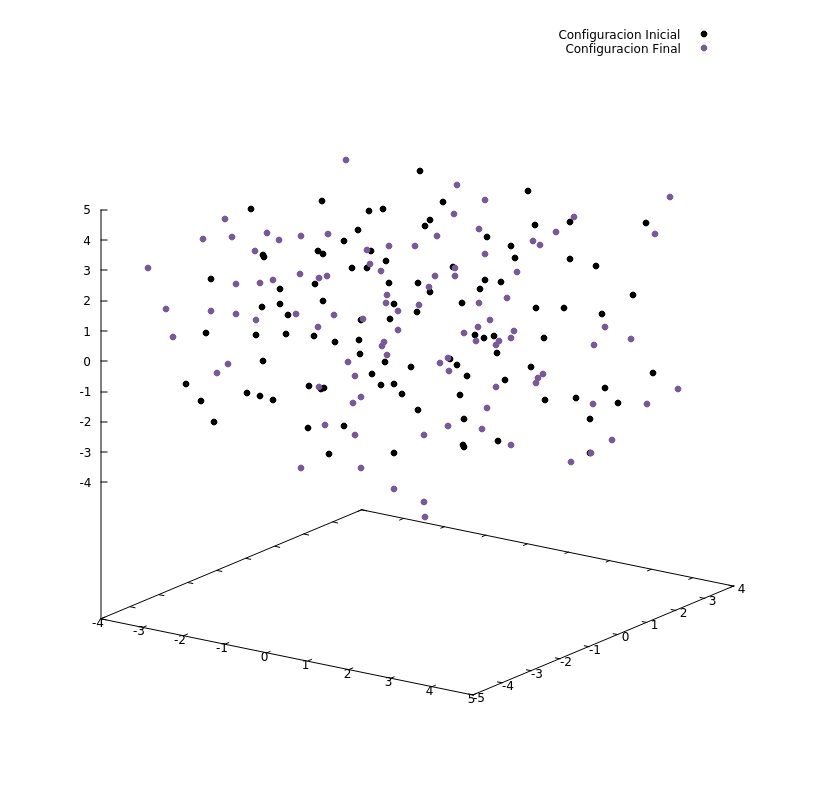
\includegraphics[width=0.5\linewidth]{ConfigS3D.png}
		\caption{ Con $n^*=0.1910$, con un $NStep=100000$ y un $\delta_{MAX}=0.5\sigma$.}
	\end{figure}
	\begin{figure}[H]
		\centering
		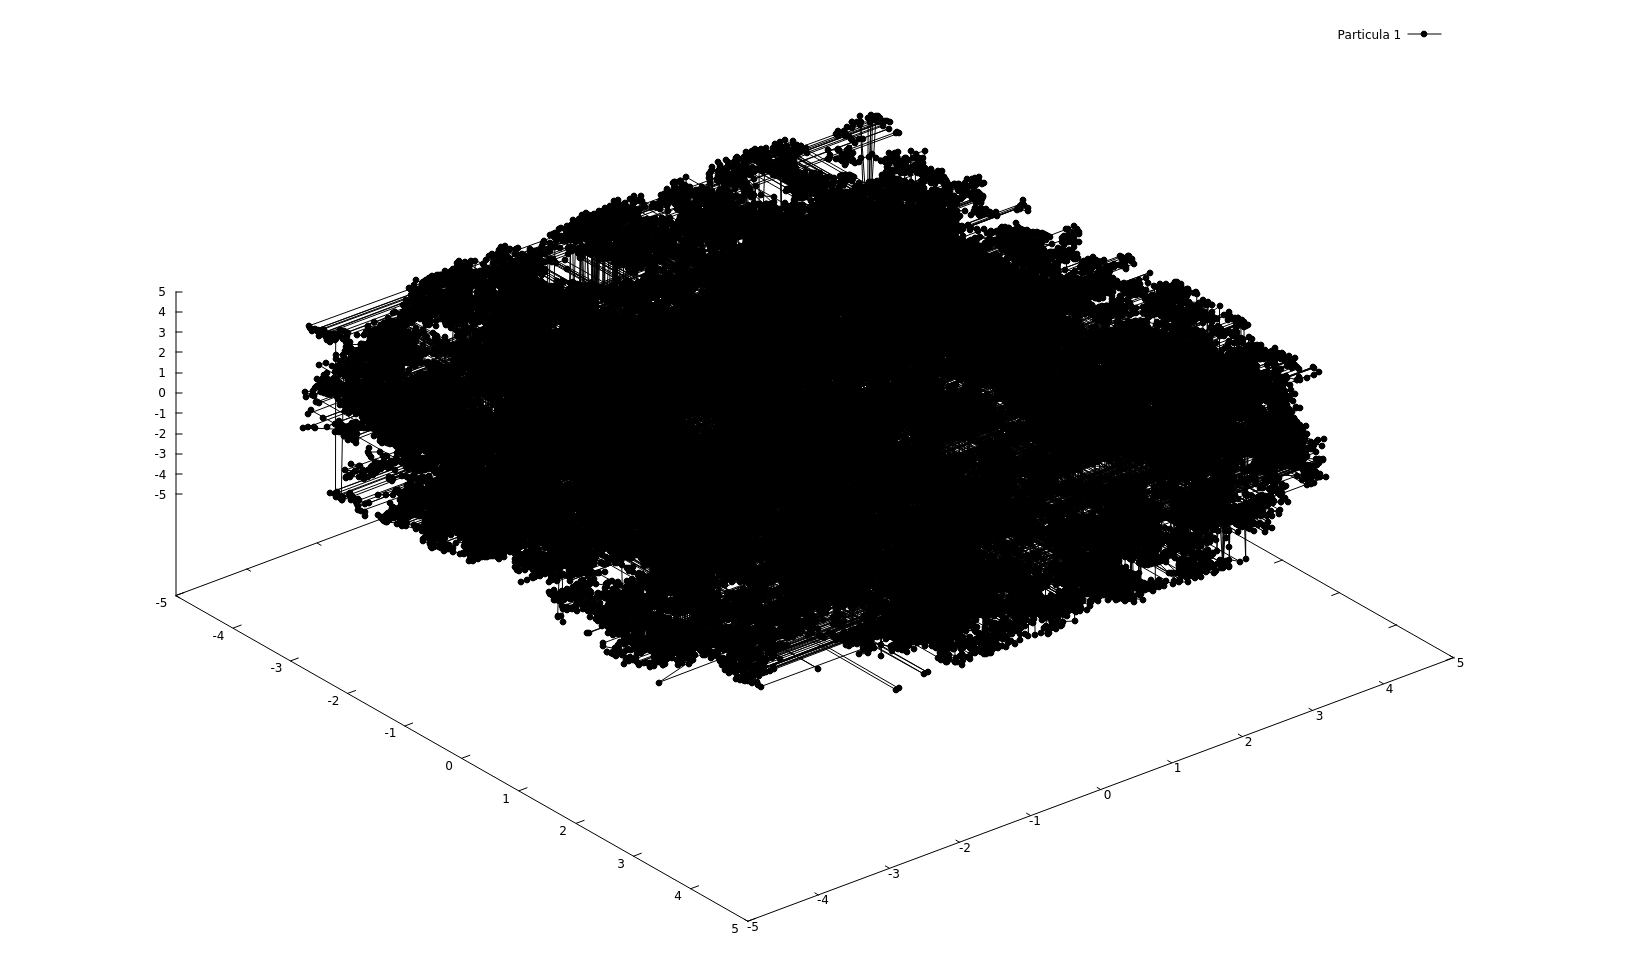
\includegraphics[width=0.49\linewidth]{Part1.png}
		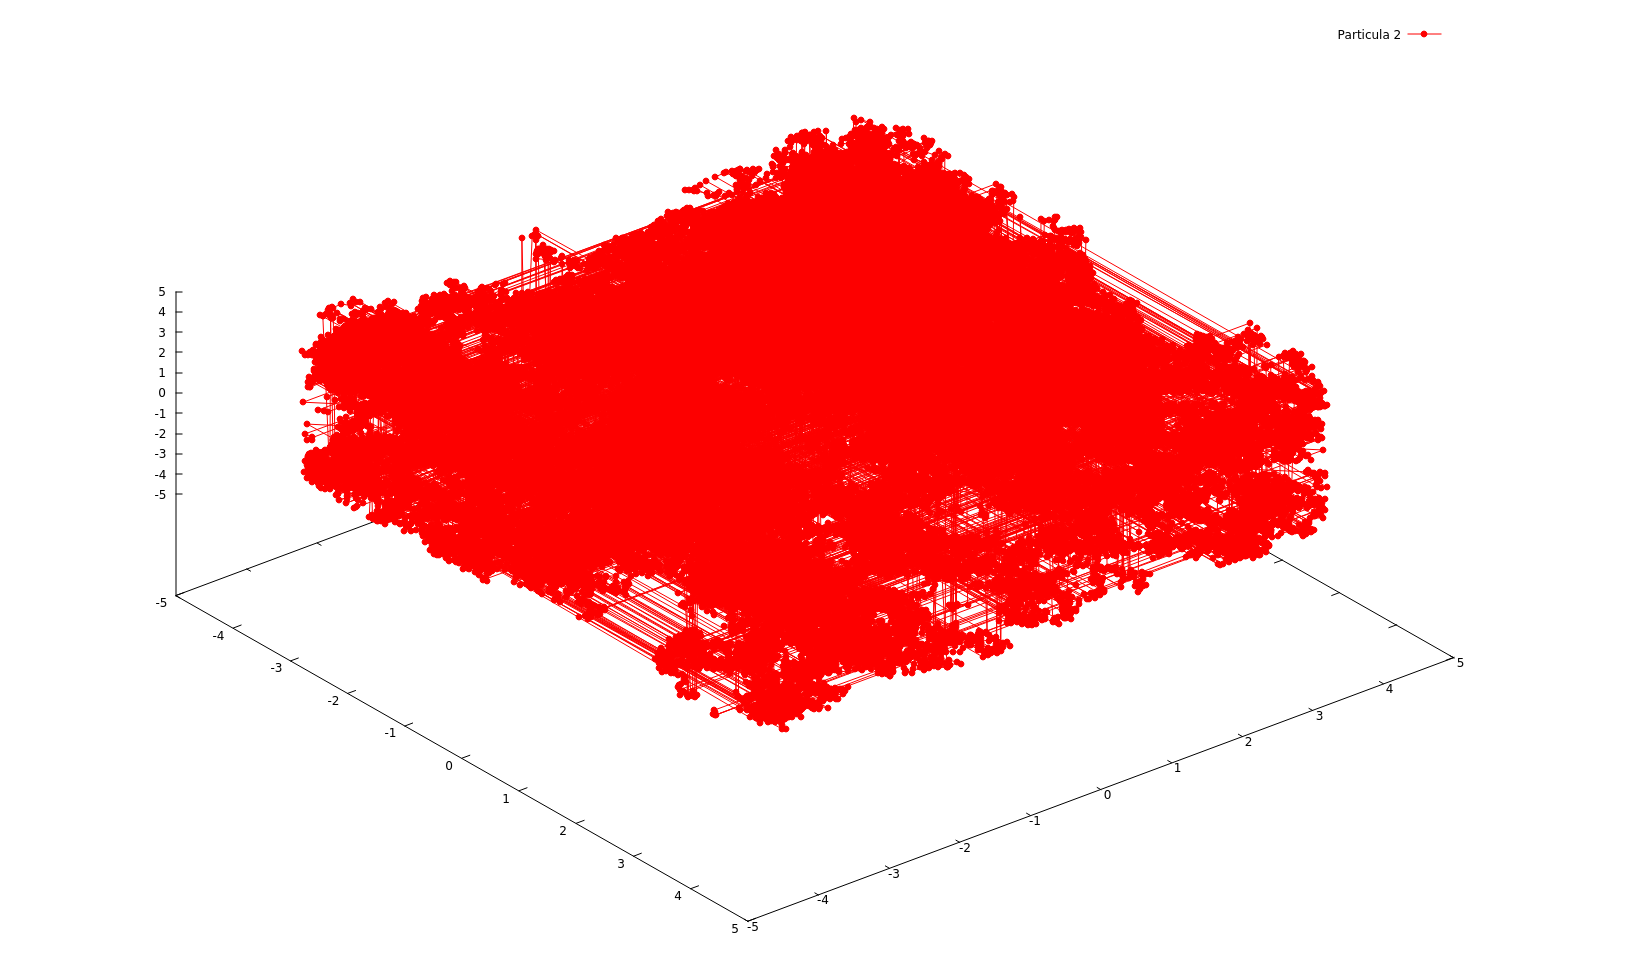
\includegraphics[width=0.49\linewidth]{Part2.png}
		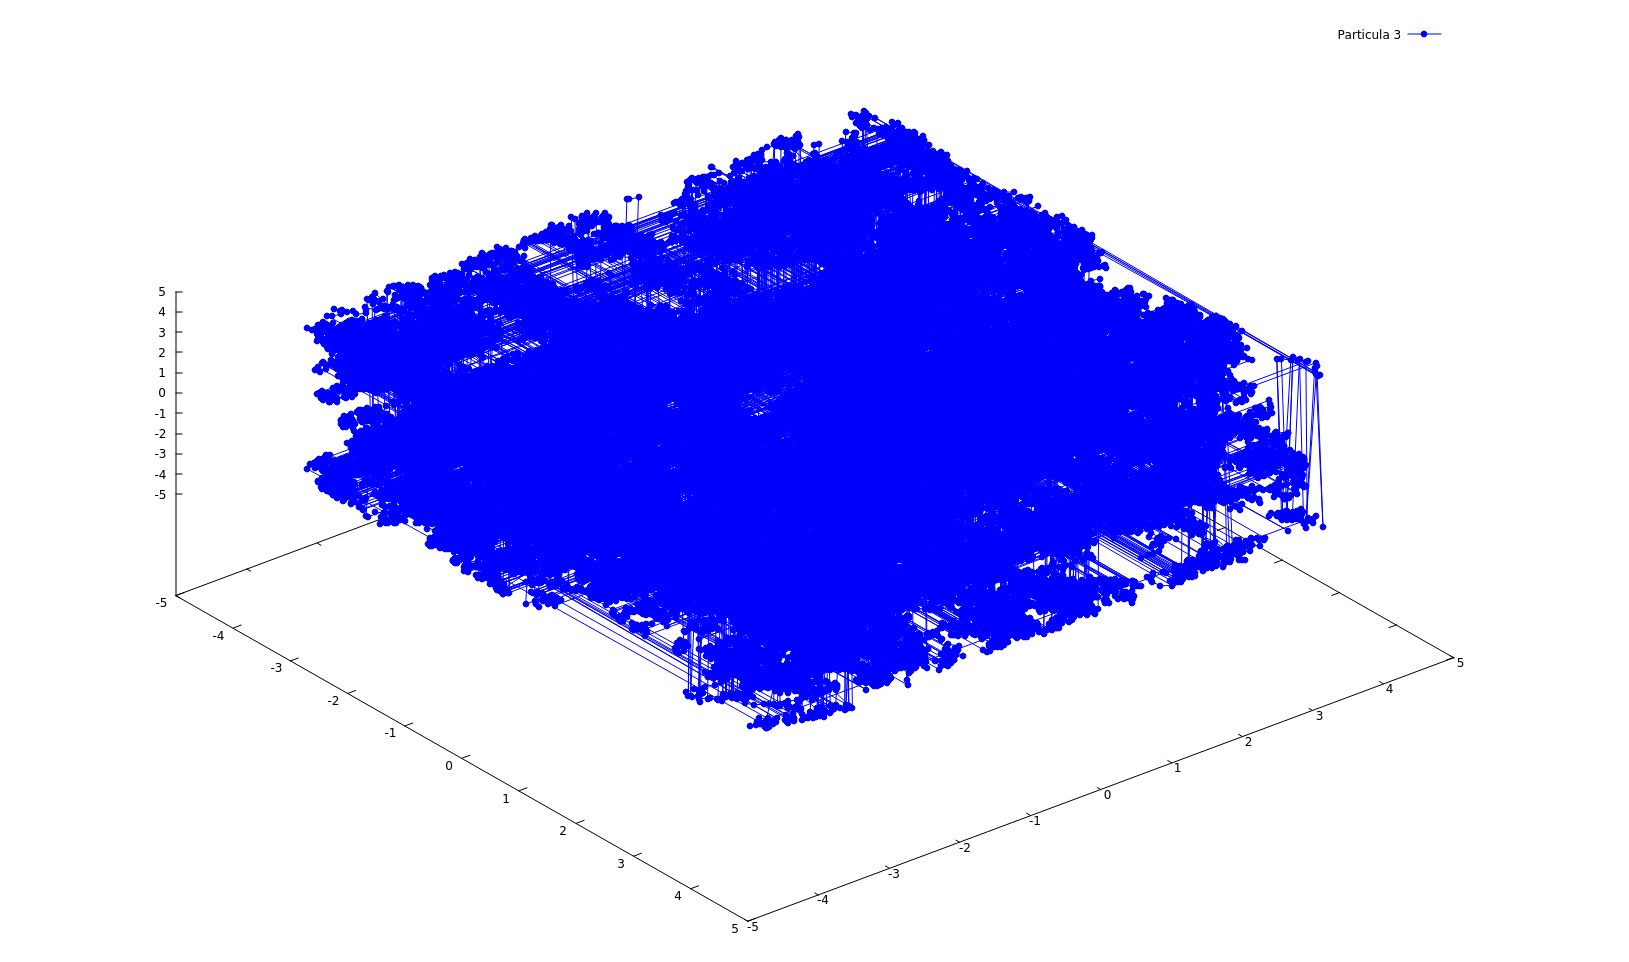
\includegraphics[width=0.49\linewidth]{Part3.png}
		\caption{Con $n^*=0.1910$, con un $NStep=100000$ y un $\delta_{MAX}=0.5\sigma$. Se realizo la traza de las partículas 84, 57 y 4.}
	\end{figure}
Se observa las configuraciones inicial y final de un arreglo en 3D. Las trazas de las partículas se aprecia algo parecido a la de la actividad 3 por las condiciones periódicas.

\subsection*{Actividad 5}
	\begin{figure}[H]
		\centering
		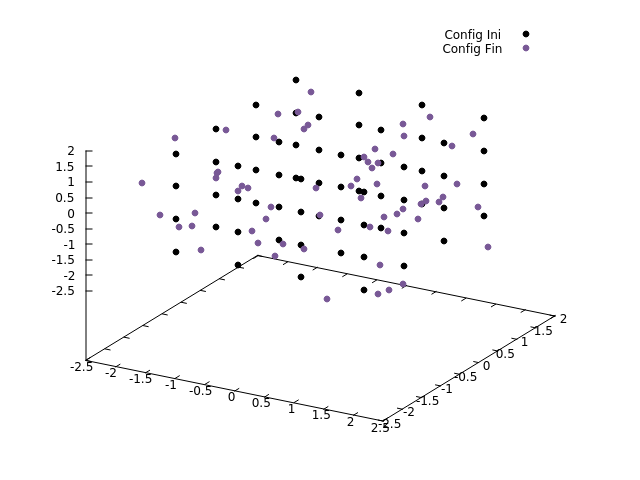
\includegraphics[width=0.5\linewidth]{ConfigS.png}
		\caption{ Con $n^*=1.0$, con un $NStep=1000$ y un $\delta_{MAX}=0.5\sigma$.}
	\end{figure}
	\begin{figure}[H]
		\centering
		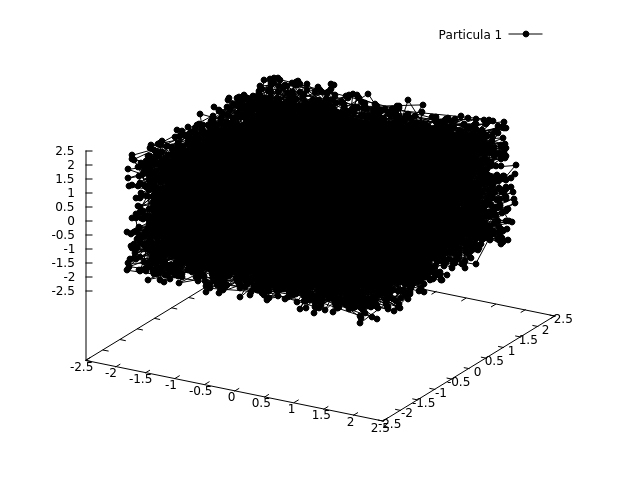
\includegraphics[width=0.49\linewidth]{Parti1.png}
		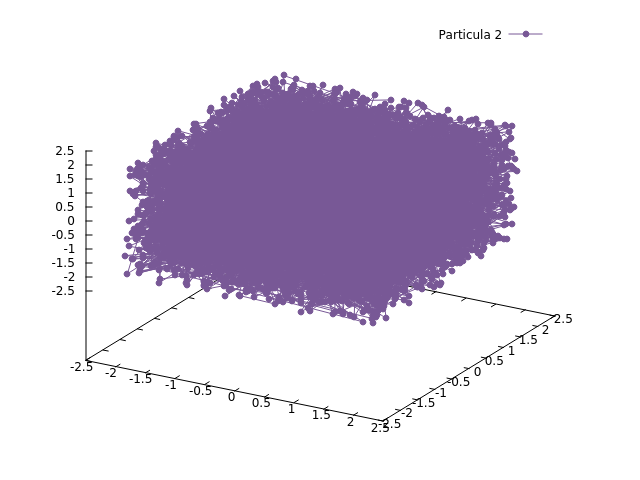
\includegraphics[width=0.49\linewidth]{Parti2.png}
		\caption{Con $n^*=1.0$, con un $NStep=1000$ y un $\delta_{MAX}=0.5\sigma$. Se realizo la traza de las partículas 64 y 36.}
	\end{figure}
	
	En la actividad se utilizó una configuración regular cúbica  en lugar de una aleatoria. y se observan las mismas cosas.
	
	\subsection*{Actividad 6}
	En esta actividad se realizo el cálculo de la energía de un sistema de disco duros (HD). Se obtuvo lo siguiente.
	\begin{figure}[H]
		\centering
		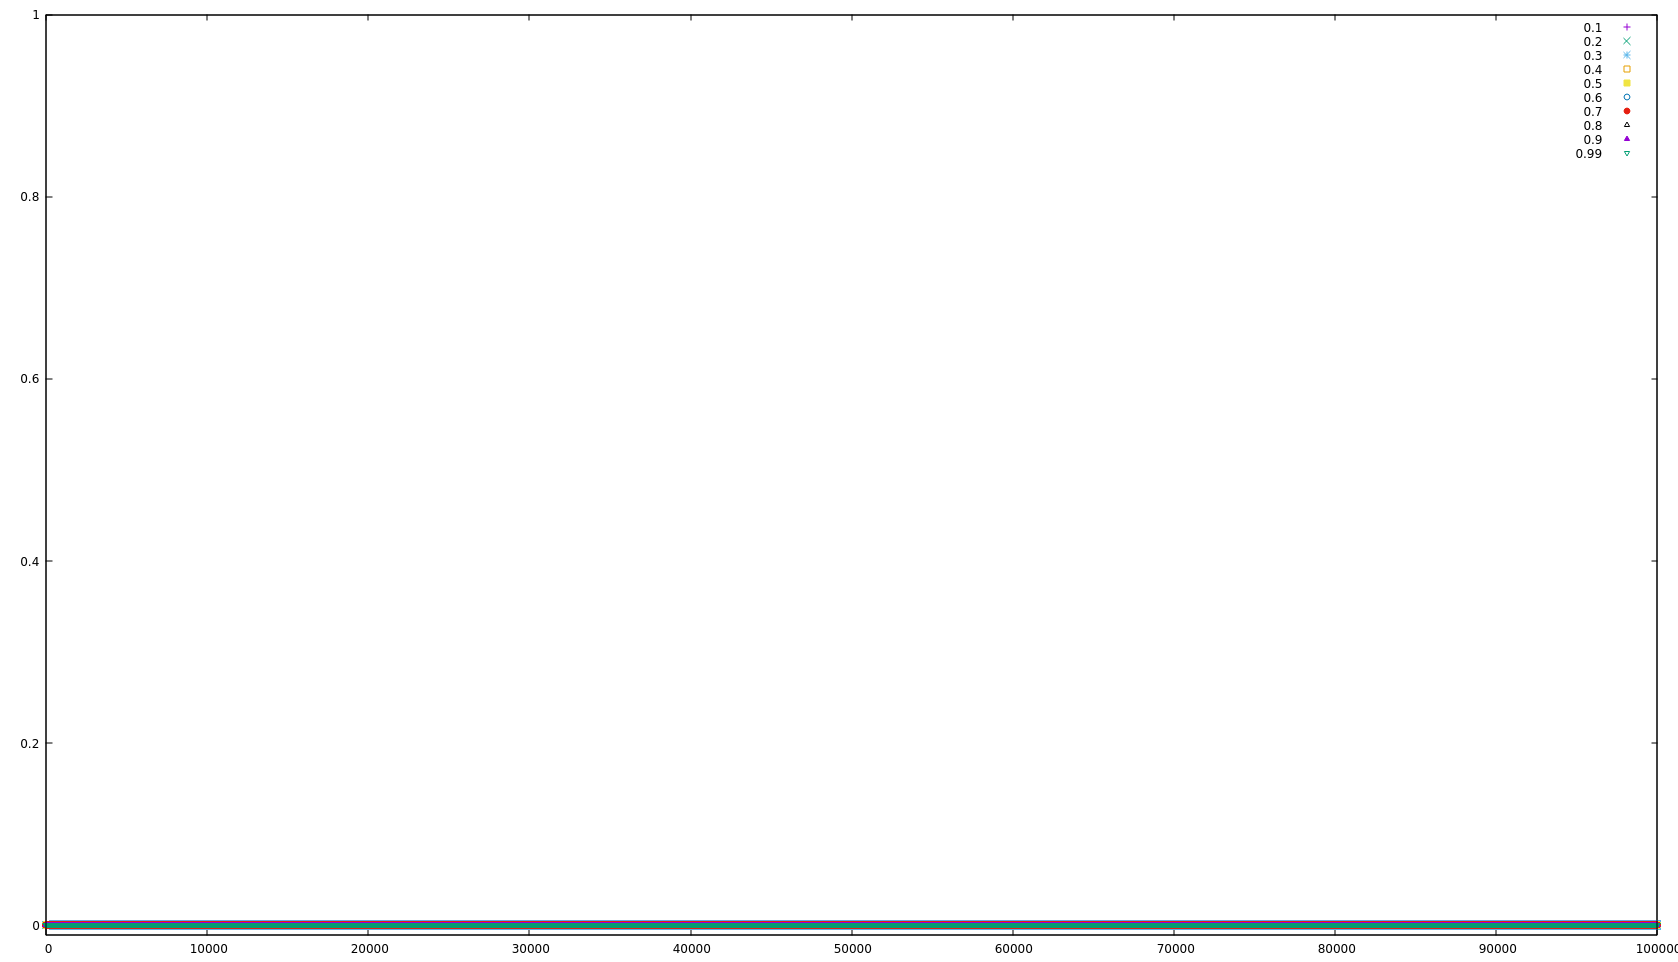
\includegraphics[width = 0.75\linewidth]{Terma.png}
		\caption{Termalización de HD para concentraciones de 0.1 a 0.99}
	\end{figure}
	Como es el potencial de discos duro, todas las configuraciones tuvieron energía 0 como era de esperarse.
\pagebreak
\section*{Tarea IV: Ejecución de Código Monte Carlo }
La tarea 4 consiste de una actividad, en la cual se implementó el código de Montecarlo.
\subsection*{Actividad 7}
Lo que se realizó en la actividad fue generar lo archivos que nos permiten observar como se va comportando la energía conforme pasan las configuraciones. El objetivo de este observar cuando un sistema se termaliza, es decir, cuando este alcanza un estado de equilibrio.

Se realizaron corridas de la simulación de Monte Carlo para las concentraciones de $n^* = 0.1$ y para la de $n^* = 0.5$, con $10,000$ configuraciones y $100$ partículas. Se escogieron estas ya que se nos pide realizar estas corridas para configuraciones  iniciales diferentes, pero para altas concentraciones la configuración aleatoria sin traslapes, suele tomar mucho tiempo o no se puede llegar a una que cumpla con las condiciones.

Empezando para la configuración aleatoria sin traslapes, llegamos a lo siguiente:

\begin{figure}[H]
	\centering
	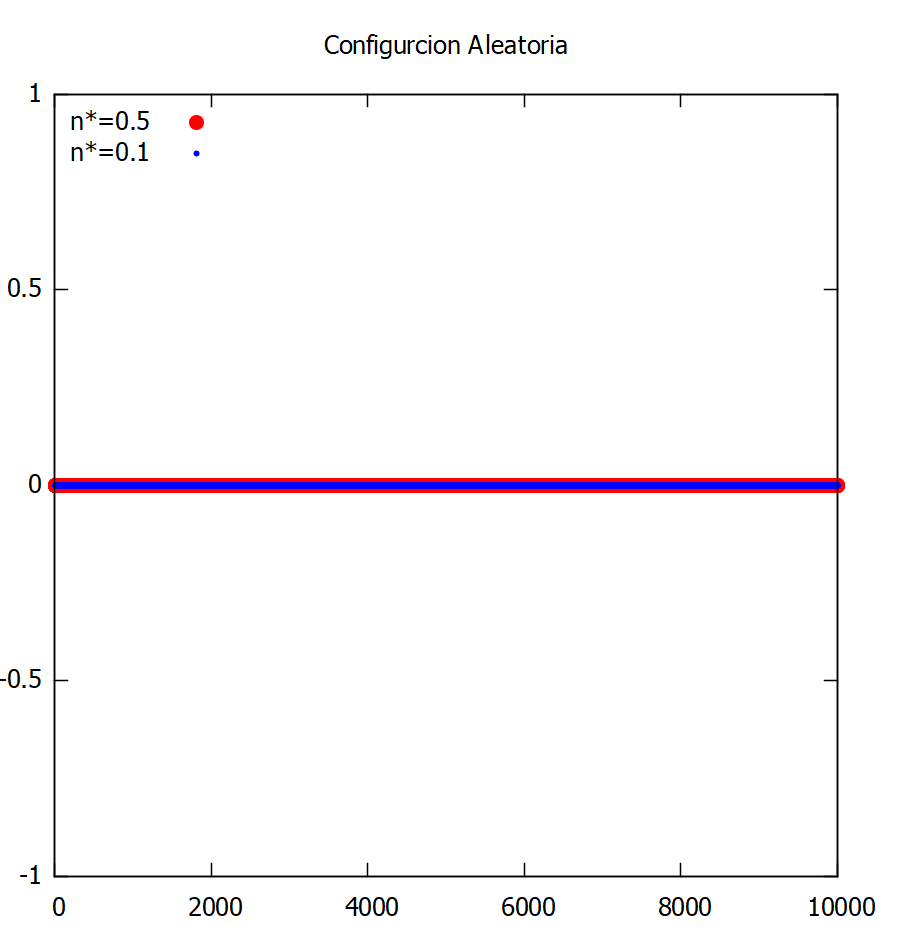
\includegraphics[width=0.5\linewidth]{aleatoria.png}
	\caption{Termalización  de simulación Monte Carlo con configuración Inicial Aleatoria para concentraciones de 0.1 y 0.5}
	\label{TermaAleatoria}
\end{figure}


Para la configuración regular, llegamos a lo siguiente:

\begin{figure}[H]
	\centering
	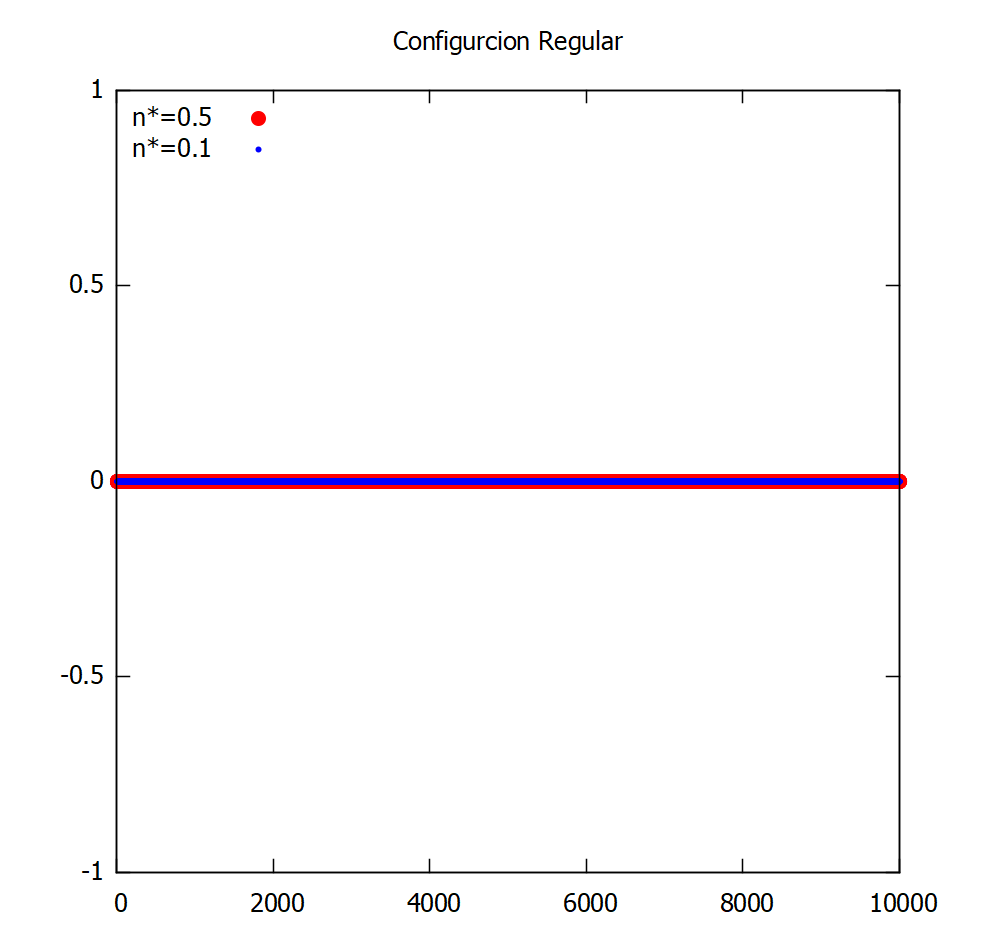
\includegraphics[width=0.5\linewidth]{regular.png}
	\caption{Termalización  de simulación Monte Carlo con configuración Inicial Regular para concentraciones de 0.1 y 0.5}
	\label{TermaReg}
\end{figure}


Podemos apreciar que la energía en ambas siempre es cero como es de esperarse, ya que para que la energía aumente en el sistema, la partículas  se deberían encontrar traslapadas, es decir que estas al colisionar no fueran duras.

Para la configuración aleatoria con traslapes es otra historia, ya que al permitir que estas se encuentre encimadas, el sistema comienza con mucha energía. Lo obtenido fue lo siguiente.

\begin{figure}[H]
	\centering
	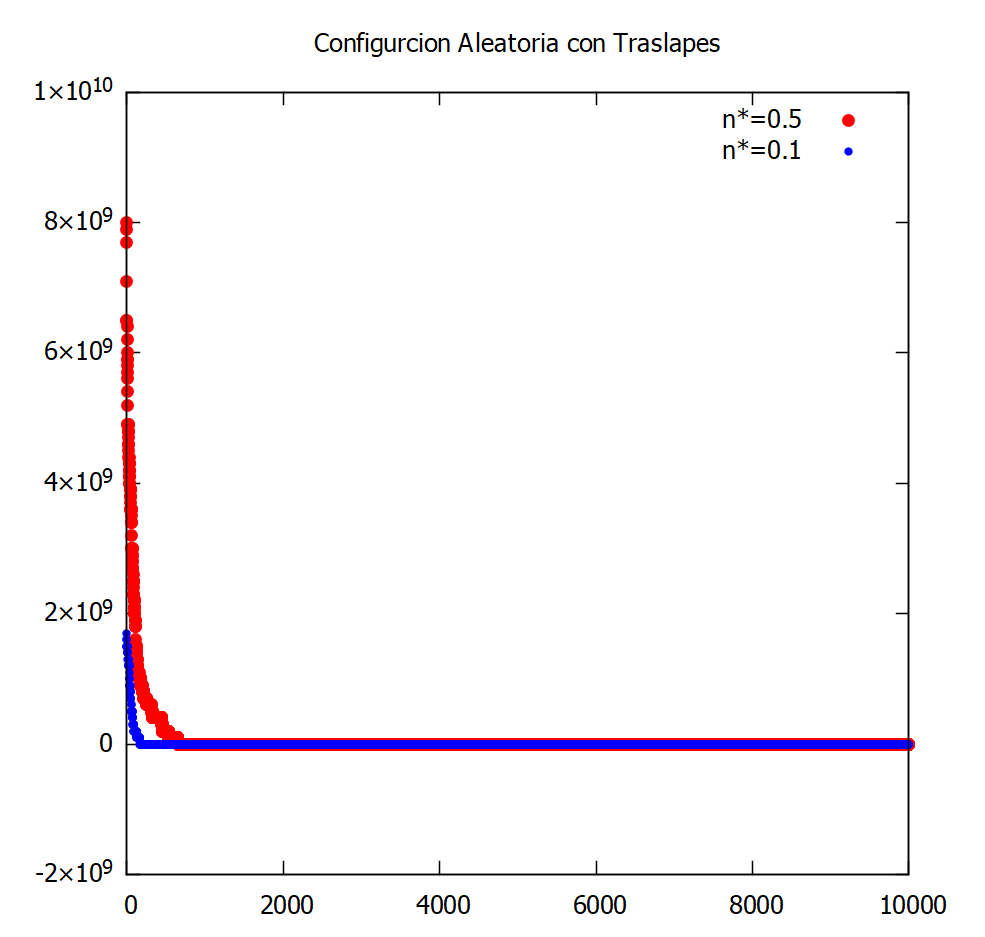
\includegraphics[width=0.50\linewidth]{traslapes.png}
	\caption{Termalización  de simulación Monte Carlo con configuración Inicial Aleatoria con Traslapes para concentraciones de 0.1 y 0.5}
	\label{TermaTras}
\end{figure}
 Se aprecia que gracias al Monte Carlo la energía disminuye, pero se observo que ambos casos la energía nunca que llego a cero que para el caso de $n^*=0.5$ la energía por partícula se estabilizó en $-184.320007$ , mientras que para $n^*=0.1$ se estabilizó en $143.360001$.
 
 Esto me permite decir que las configuraciones que inician con traslapes no son tan confiables para este caso de estudió.

 \pagebreak

\section*{Tarea V: Propiedades	Estructurales	de	un	Sistema	de	Discos	Duros}
Esta tarea consistió en observar las gráficas de las G(r) y como se altera con los diferente parámetros en la simulación.

\subsection*{Actividad 8: G(r) bajo diferentes parámetros}
Lo primero que  se realizó fue realizar una simulación con diferentes configuraciones iniciales. Estas se realizaron para concentraciones de $n^*=0.5$ y con  $30,000$ configuraciones y 100 partículas.

\begin{figure}[H]
	\centering
	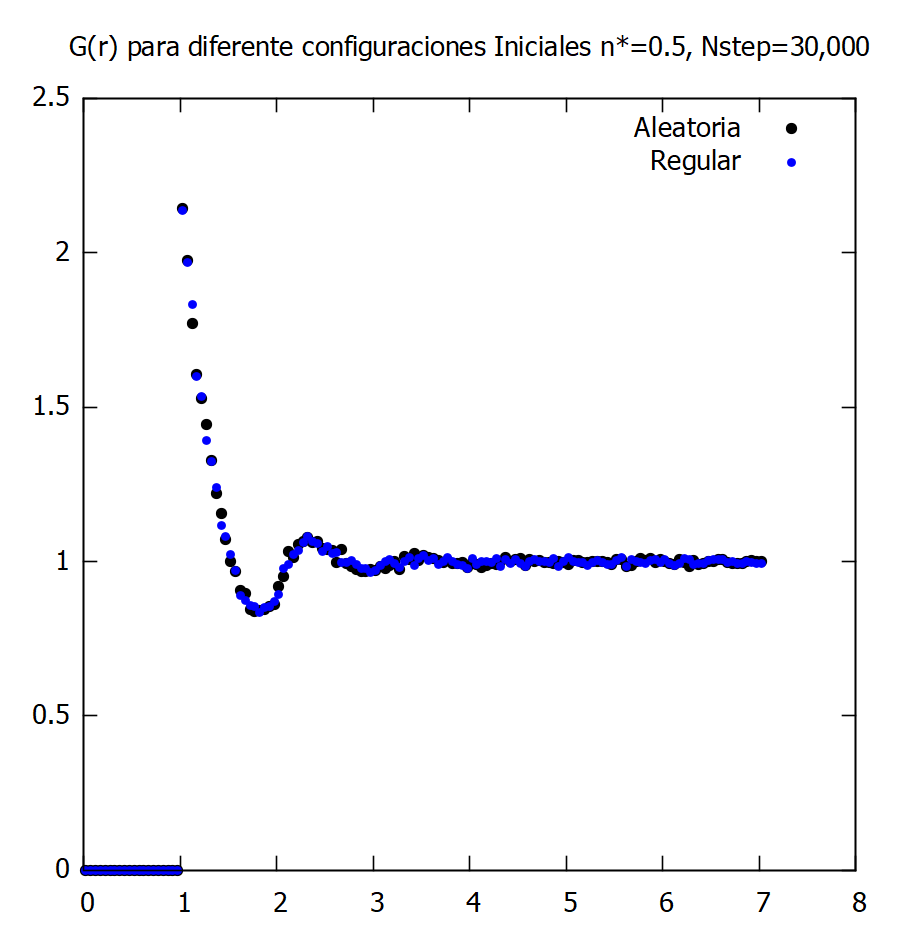
\includegraphics[width=0.50\linewidth]{gdrCNF.png}
	\caption{Distribución Radial para diferentes configuraciones iniciales}
	\label{GDR_Config}
\end{figure}

Luego se realizó variando el numero de partículas bajo las misma condiciones.

\begin{figure}[H]
	\centering
	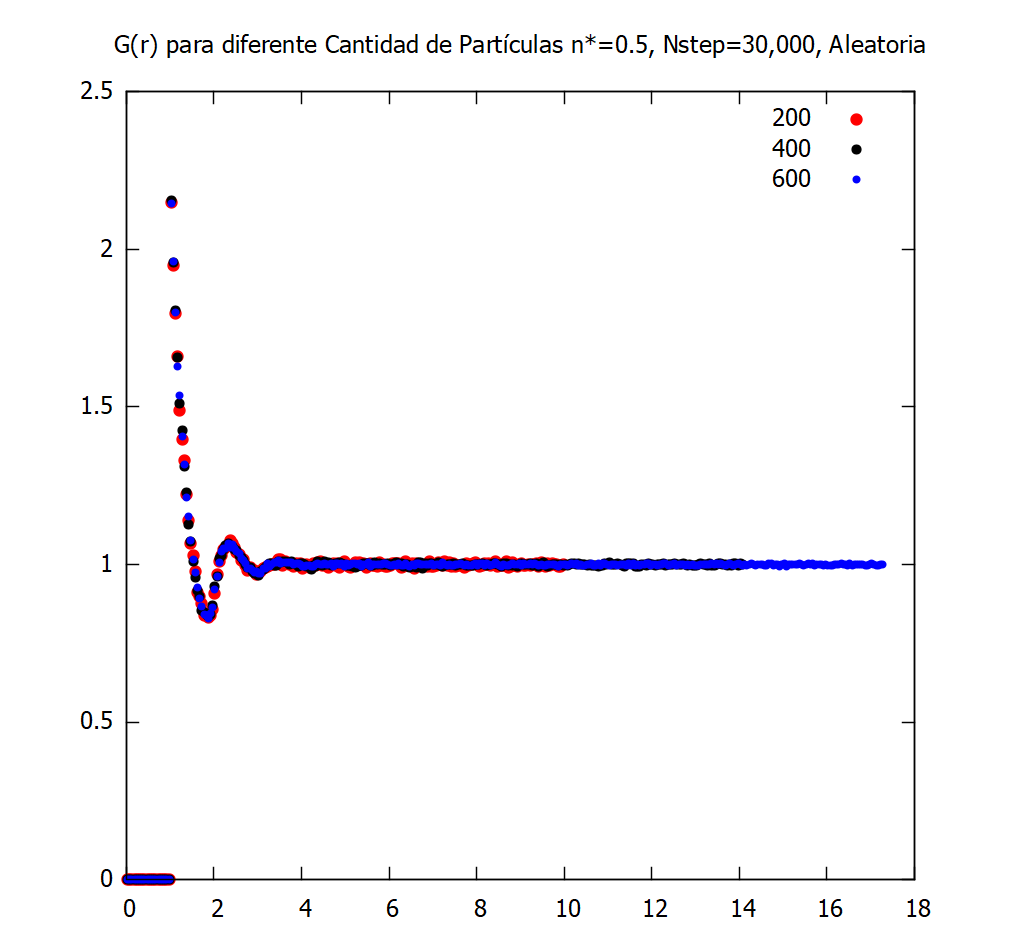
\includegraphics[width=0.50\linewidth]{gdrPart.png}
	\caption{Distribución Radial para diferente numero de partículas}
	\label{GDR_Particulas}
\end{figure}

Finalmente se realizó para un deltar diferente y mismas condiciones que al principio.

\begin{figure}[H]
	\centering
	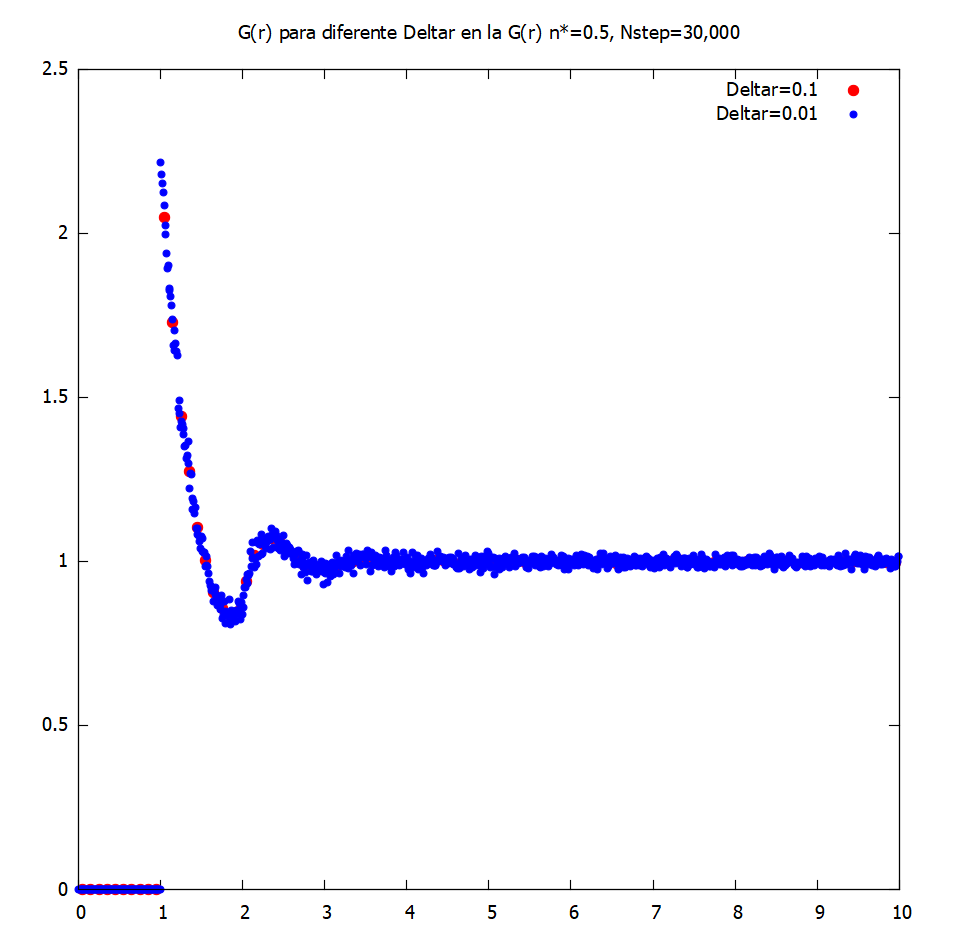
\includegraphics[width=0.50\linewidth]{gdrDeltar.png}
	\caption{Distribución Radial para deltar diferentes}
	\label{GDR_Deltar}
\end{figure}
 En figura \ref{GDR_Config} nos muestra que la configuración aleatoria tiene mejor comportamiento, esto se debe a que la regular no ha olvidado la configuración inicial. La figura \ref{GDR_Particulas} se observa que entre más partículas, existen mas datos para realizar el calculo de la distribución radial. La figura \ref{GDR_Deltar} nos muestra que un deltar pequeño puede llegar a generar mas ruido y es mas recomendable que no se ni muy pequeño ni muy grande.
 
 \subsection*{Actividad 9: Densidad	local de partículas}
La función de distribución nos permite obtener un estimado de cuantas partículas consistió la simulación. Lo que se realizó fue tomar los archivos de la gdr de la actividad anterior para diferente numero de partículas.

Nuestros resultados fueron los siguientes:
\begin{table}[H]
	\centering
	\begin{tabular}{|c|c|}
		\hline 
		N (Entrada) & N  ( g(r) ) \\ \hline 
		200 & 198.77 \\ \hline 
		400 & 396.39 \\ \hline 
		600 & 597.36 \\ \hline 
	\end{tabular} 
	\caption{Número de partículas.\\ El que se dio de entrada y el que se calcula.}
	\label{N_Particulas}
\end{table}	

\subsection*{Actividad 10: Función de correlación radial g(r) para las  concentraciones reducidas}	

Lo que se busca es observar el comportamiento que tiene la g(r) con la variación de la concentración. Se realizaron corridas para las concentraciones de $n^* = 0.01$, $n^*=0.1$, $n^*=0.3$, $n^*=0.5$, $n^*=0.7$, $n^*=0.9$ y $n^*=0.999$

Los resultados fueron lo siguientes:
\begin{figure}[H]
	\centering
	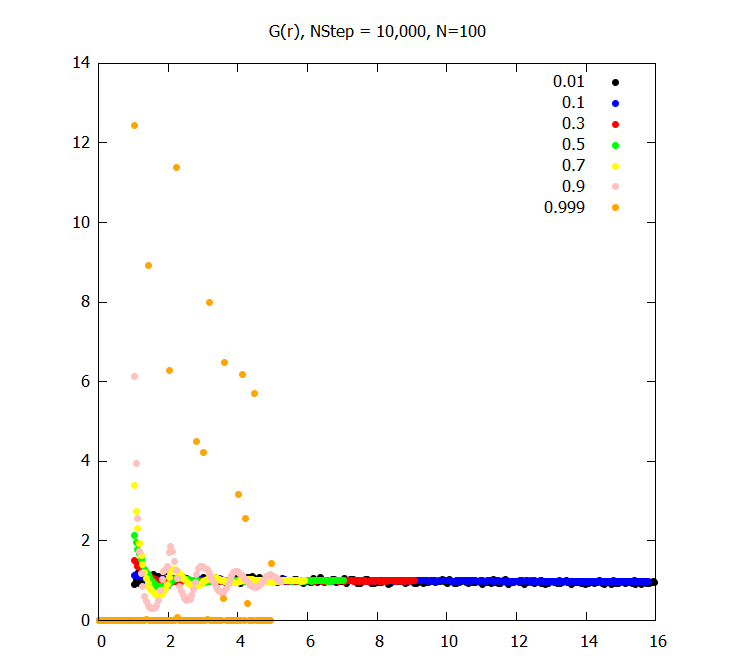
\includegraphics[width=0.50\linewidth]{gdrT.png}
	\caption{Distribución Radial para diferente concentraciones}
	\label{GDR_Cons}
\end{figure}
Se observa que a bajas concentraciones no alcanza a tomar forma ya que las partículas se encuentran alejadas. Para la concentración de $n^*=0.999$ no alcanzo a olvidar la configuración inicial regular, lo que explica su forma.

La termalización fue la siguiente:
\begin{figure}[H]
	\centering
	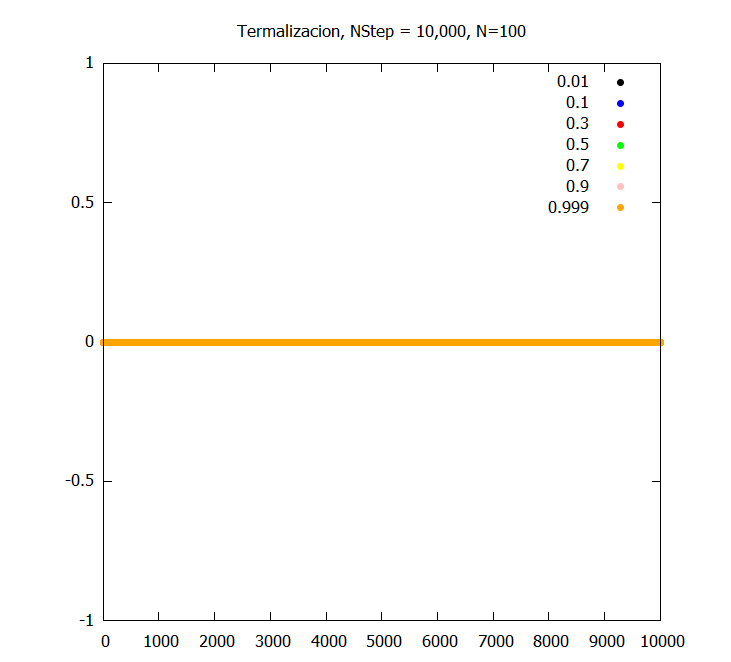
\includegraphics[width=0.50\linewidth]{TermaT.png}
	\caption{Termalización para diferente concentraciones}
	\label{Term_Cons}
\end{figure}
Como era de esperarse la energía siempre fue 0.


\subsection*{Actividad 11: Ecuación de Estado}

Lo que se realizó fue calcular la presión del sistema a partir de los archivos de la GDR. Se tomaron los archivos de la actividad anterior y se procedió a calcular la presión.

Los resultados fueron los siguientes
\begin{figure}[H]
	\centering
	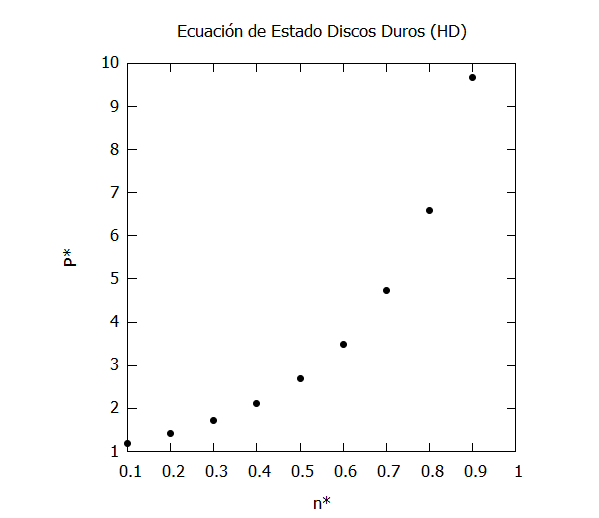
\includegraphics[width = 0.5\linewidth]{EcEstado.png}
	\caption{Ecuación de Estado para discos duros (HD)}
\end{figure}


\section*{Código Utilizado}
\lstinputlisting[caption={Codigo del Modulo de Variables Globales}]{Mod.f03}
%caption={Código ErrorRe.py}

\end{document}

